% Se puede cambiar a [11pt] si el docente lo requiere, por defecto es 12pt.
\documentclass[12pt]{catolica_proyectos}
\addbibresource{bibliografia.bib}
% --- DATOS DEL PROYECTO ---
\titulo{Diseño de un Sistema de Monitoreo de Signos Vitales de Bajo Costo}
\materia{Sensores y Transductores}
\carrera{Mecatrónica} % Mecatrónica, Sistemas o Biomédica
\autor{Nombre del Estudiante}
\docente{Ing. profesor}
\semestre{1/2026}

\begin{document}
	
	\maketitle
	\pagestyle{empty}
	\tableofcontents
	\newpage
	
	\listoffigures   % Índice de figuras
	\newpage
	
	\listoftables    % Índice de tablas
	\newpage
	
	\pagenumbering{arabic} 
	\setcounter{page}{1}
	
	\section{Descripción técnica-conceptual del proyecto a realizar}
	
	El objetivo es que el lector, en una o dos páginas, exponga de qué se trata el proyecto y cuáles son sus desafíos, cuál es la motivación para realizarlo y su importancia.
	
	Se debe introducir el contexto del proyecto, el estado del arte en la temática, describir la propuesta de valor, cuál es el problema que atiende y cuál es la solución que se propone. Se debe dar una descripción funcional de la solución que incluya un diagrama en bloques.
	La descripción técnica-conceptual \textbf{debe incluir al menos un diagrama en bloques del sistema} y descripción funcional de la solución propuesta.
	
	Las figuras se deben mencionar en el texto ANTES de que aparezcan con una frase como la siguiente: ``En la figura \ref{fig:diagBloques} se presenta el diagrama en bloques del sistema. Se observa que...''.  La regla es que las figuras nunca pueden ir antes de ser mencionadas en el texto, porque sino el lector no entiende por qué de pronto aparece una figura.
	
	
	\begin{figure}[htpb]
		\centering 
		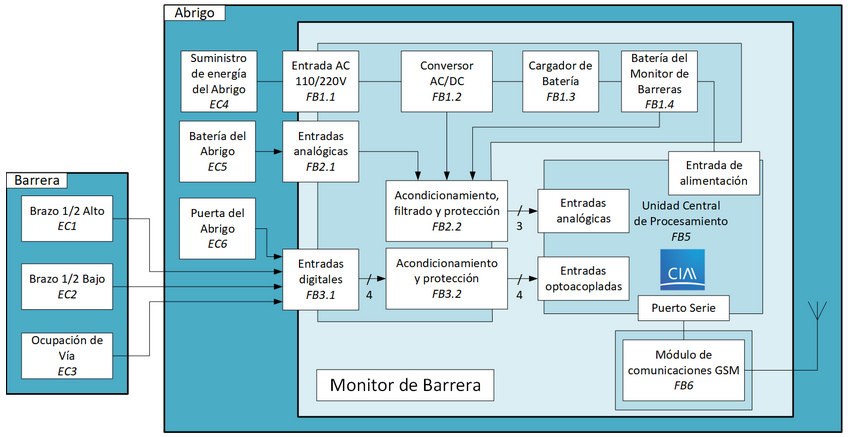
\includegraphics[width=.65\textwidth]{./Figuras/diagBloques.png}
		\caption{Diagrama en bloques del sistema.}
		\label{fig:diagBloques}
	\end{figure}
	
	
	\section{Propósito del proyecto}
	
	¿Por qué se hace el proyecto? ¿Qué se quiere lograr? 
	
	
	\section{Alcance del proyecto}
	
	¿Qué se incluye y que no se incluye en este proyecto?
	
	Se refiere al trabajo que se va a hacer para entregar el producto o resultado especificado. 
	
	Explicitar todo lo quede comprendido dentro del alcance del proyecto. Por ejemplo:
	
	El proyecto incluye:
	\begin{itemize}
		\item Ítem 1.
		\item Ítem 2.
		\begin{itemize}
			\item Subítem 1.
			\item Subítem 2.
			\item ...
		\end{itemize}
		\item ...
		
	\end{itemize}
	
	Explicitar además todo lo que no quede incluido (``El presente proyecto no incluye...'')
	
	\section{Supuestos del proyecto}
	
	``Para el desarrollo del presente proyecto se supone que: ...''
	
	\begin{itemize}
		\item Supuesto 1.
		\item Supuesto 2.
		\item ...
	\end{itemize}
	
	Por ejemplo, se podrían incluir supuestos respecto a disponibilidad de tiempo y materiales, sobre la factibilidad técnica de distintos aspectos del proyecto, sobre otras cuestiones que sean necesarias para el éxito del proyecto.
	
	
	\section{Requerimientos}
	
	Los requerimientos deben enumerarse y de ser posible estar agrupados por afinidad, por ejemplo:
	
	\begin{enumerate}
		\item Requerimientos funcionales:
		\begin{enumerate}
			\item El sistema debe...
			\item Tal componente debe...
			\item El usuario debe poder...
		\end{enumerate}
		\item Requerimientos de documentación:
		\begin{enumerate}
			\item Requerimiento 1.
			\item Requerimiento 2 (prioridad menor)
		\end{enumerate}
		\item Requerimiento de testing...
		\item Requerimientos de la interfaz...
		\item Requerimientos interoperabilidad...
		\item etc...
	\end{enumerate}
	
	Leyendo los requerimientos se debe poder interpretar cómo será el proyecto y su funcionalidad.
	
	
	\section{Entregables principales del proyecto}
	
	Los entregables del proyecto son (ejemplo):
	
	\begin{itemize}
		\item Manual de usuario.
		\item Diagrama de circuitos esquemáticos.
		\item Código fuente del firmware \cite{ucb2026}.
		\item Diagrama de instalación \cite{doe2024}.
		\item Memoria del trabajo final.\cite{ogata2010}
		\item etc...
	\end{itemize}
	
	% --- Bibliografía APA 7ma Edición ---
	\newpage
	% Usamos el heading predefinido bibintoc para que salga en el índice sin errores de macros
	\printbibliography[heading=bibintoc, title={Referencias Bibliográficas}]
		
\end{document}